\documentclass[10pt,landscape]{exam}
\usepackage[phy]{template-for-exam}
\usepackage[margin=0.4in]{geometry}
\usepackage{multicol,silence,graphicx}

\WarningFilter{latex}{Label `question}
\WarningFilter{latex}{There were multiply-defined labels}
\WarningFilter{latex}{Label `part}
%%%%%%%%%%%%%%%%%%%%%%%%%%%%%%%%%%%%%

\def\todayDate{Mon, May 11}

\def\content{
Write a paragraph (3-4 sentences) explaining how a satellite dish allows for enhanced reception of radio waves.  Make sure to use the following vocabulary terms in your paragraph: 

\begin{multicols*}{2}
  \begin{itemize}
    \item concave mirror
    \item focal point
    \item reflection / reflect
    \item diffuse reflection
    \item wavelength 
  \end{itemize}

  \vfill
  \columnbreak

  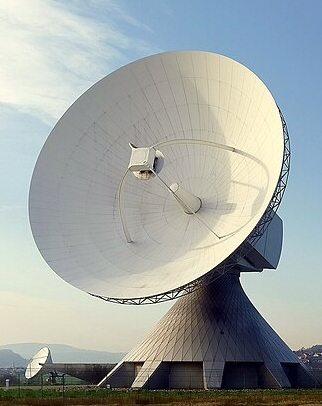
\includegraphics[width=4cm]{SatelliteDish.jpg}
\end{multicols*}

}

%%%%%%%%%%%%%%%%%%%%%%%%%%%%%%%%%%%%%%

\begin{document}
\pagestyle{empty}

\setlength{\columnsep}{0.8in}
\begin{multicols*}{2}

\noindent  
Name: \hfill Period: \hspace{5em}
\vspace{0.5em}
\hrule

\section*{\todayDate}
\subsection*{Warmup}

\content

\vfill
\hrule
\vspace{0.5em}
\hfill {\sc Physics I}

\columnbreak

\noindent  
Name: \hfill Period: \hspace{5em}
\vspace{0.5em}
\hrule

\section*{\todayDate}
\subsection*{Warmup}

\content

\vfill
\hrule
\vspace{0.5em}
\hfill {\sc Physics I}

\end{multicols*}

\end{document}